\documentclass[11pt]{article}
\usepackage{amsmath, amssymb}
\usepackage{tikz}
\usetikzlibrary{positioning, calc, arrows.meta}
\usepackage{booktabs}
\usepackage[margin=1in]{geometry}
\usepackage{parskip}
\usepackage{enumitem}
\setlist{itemsep=2pt, topsep=2pt}

\title{Lecture Notes: Steady-State Error\\
       \large Week 6 --- ME 2801}
\author{}
\date{}

\begin{document}
\maketitle

\section*{The Question}

After the transients die out, where does the output sit relative to the
reference?  Transient analysis (week~4) tells us \emph{how} the system
gets there; steady-state error analysis tells us \emph{where} it ends up.

Two performance dimensions, distinct and complementary:

\begin{center}
\begin{tabular}{ll}
\toprule
Transient (week 4)        & Steady state (week 6) \\
\midrule
Settling time, overshoot  & Final offset, ramp lag \\
Damping ratio             & Persistent tracking error \\
Pole locations            & DC behavior of the loop \\
\bottomrule
\end{tabular}
\end{center}

\section*{Setting and Assumptions}

\begin{figure}[h]
\centering
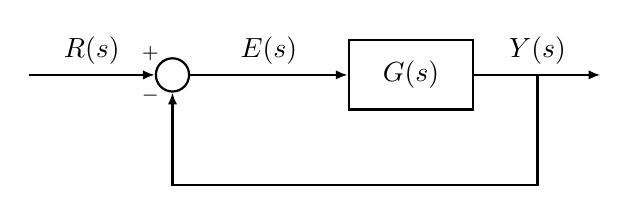
\begin{tikzpicture}[
  >={Latex[length=1.5mm, width=1.2mm]}, thick,
  block/.style = {draw, rectangle, minimum height=2.5em, minimum width=4.5em},
  sum/.style   = {draw, circle, inner sep=0pt, minimum size=1.2em},
]
  \node[coordinate]                   (rin)  {};
  \node[sum,   right=1.6cm of rin]    (sum)  {};
  \node[block, right=2.0cm of sum]    (G)    {$G(s)$};
  \node[coordinate, right=1.6cm of G] (yout) {};

  \node[font=\scriptsize, inner sep=0pt, anchor=south east] at (sum.north west) {$+$};
  \node[font=\scriptsize, inner sep=0pt, anchor=north east] at (sum.south west) {$-$};

  \draw[->] (rin)  -- node[above]{$R(s)$} (sum);
  \draw[->] (sum)  -- node[above]{$E(s)$} (G);
  \draw[->] (G)    -- node[above]{$Y(s)$} (yout);

  \coordinate (fbk) at ($(G.east)!0.5!(yout)$);
  \draw[->] (fbk) -- ++(0,-1.4) -| (sum.south);
\end{tikzpicture}
\end{figure}

\textbf{Unity negative feedback}, with $G(s) = C(s)\,P(s)$ the combined
open-loop forward path (controller $\times$ plant).  Two preconditions
that the formulas silently rely on:

\begin{enumerate}
  \item The closed loop is \textbf{stable}.  Without this, the final value
    theorem does not apply and the answer is meaningless.
  \item The error signal is $E(s) = R(s) - Y(s)$, formed at the summing
    junction.
\end{enumerate}

\textbf{Notation reminder.}  The symbol $G(s)$ in this article is overloaded:
elsewhere it means the plant alone.  Here, and only here, it means controller
times plant.

\section*{The Master Equation}

From $Y = GE$ and $E = R - Y$:
\[
  E(s) = \frac{R(s)}{1+G(s)}
  \qquad\Longrightarrow\qquad
  e(\infty) = \lim_{s\to 0} s\,E(s)
\]

\[
  \boxed{\;e(\infty) = \lim_{s\to 0}\,\frac{s\,R(s)}{1+G(s)}\;}
\]

Everything in the chapter follows from this single limit.  No new
derivations --- only substitution and evaluation.

\section*{Three Test Inputs}

\begin{center}
\begin{tabular}{lccl}
\toprule
Name      & $r(t)$            & $R(s)$  & Scenario \\
\midrule
Step      & $1$               & $1/s$   & Hold a fixed setpoint \\
Ramp      & $t$               & $1/s^2$ & Track a constant-velocity target \\
Parabola  & $\tfrac12 t^2$    & $1/s^3$ & Track a constant-acceleration target \\
\bottomrule
\end{tabular}
\end{center}

Defense framing: stationary target / constant-velocity target / maneuvering
target.  Each successive case demands one more integrator in the forward
path to keep error bounded.

\section*{System Type}

\textbf{Definition.}  The \emph{type} of the system is the number $n$ of
pure integrators (poles at the origin) in the open-loop forward TF:
\[
  G(s) = \frac{K\,(s+z_1)(s+z_2)\cdots}{s^n\,(s+p_1)(s+p_2)\cdots}
\]

Type is a property of the \emph{combined} forward path.  Adding $K_I/s$
to the controller bumps the type by one --- it does not matter where the
integrator lives, only that it is in the loop.

\section*{Static Error Constants}

Three limits appear so often they get names:
\begin{align*}
  K_x &= \lim_{s\to 0} G(s)        &&\text{(position)} \\
  K_v &= \lim_{s\to 0} s\,G(s)     &&\text{(velocity)} \\
  K_a &= \lim_{s\to 0} s^2\,G(s)   &&\text{(acceleration)}
\end{align*}

(We use $K_x$ instead of the textbook $K_p$ to avoid colliding with the
PID proportional gain $K_P$.)

\section*{Summary: The Diagonal Pattern}

\begin{center}
\begin{tabular}{lccc}
\toprule
         & Type 0              & Type 1              & Type 2 \\
\midrule
Step     & $\dfrac{1}{1+K_x}$  & $0$                 & $0$ \\[8pt]
Ramp     & $\infty$            & $\dfrac{1}{K_v}$    & $0$ \\[8pt]
Parabola & $\infty$            & $\infty$            & $\dfrac{1}{K_a}$ \\
\bottomrule
\end{tabular}
\end{center}

\textbf{Read the table along the diagonal:}
\begin{itemize}
  \item Above the diagonal: zero error (the system has more than enough
    integrators).
  \item On the diagonal: finite error, governed by the matching error
    constant.
  \item Below the diagonal: error diverges (not enough integrators).
\end{itemize}

A single number like ``$K_v = 20$'' encodes type, input, and error all
at once: stable, Type 1, ramp input, $5\%$ error per unit slope.

\section*{Design Recipe}

When the type is fixed by the architecture and only a forward gain $K$ is
free:
\begin{enumerate}
  \item Identify the type by inspection.
  \item Write the relevant error constant ($K_x$, $K_v$, or $K_a$) in
    terms of $K$.
  \item Solve for $K$ to meet the spec.
  \item \textbf{Verify the closed loop is still stable at that $K$.}
\end{enumerate}

\section*{Two Ways to Kill Steady-State Error}

\begin{center}
\begin{tabular}{p{3.5cm}p{5.5cm}p{5.5cm}}
\toprule
                & \textbf{Integrator (PI / I action)}
                & \textbf{Feedforward $1/K_{\mathrm{dc}}$} \\
\midrule
Mechanism       & Accumulates error until $e\to 0$.
                & Injects the steady-state effort directly. \\[4pt]
Needs a model?  & No --- self-correcting.
                & Yes --- needs accurate plant DC gain. \\[4pt]
System type     & $+1$.
                & Unchanged. \\[4pt]
Disturbances    & Rejects them.
                & Does not see them. \\[4pt]
Cost            & Slower settling, possible overshoot, windup.
                & Residual error if the model is wrong. \\
\bottomrule
\end{tabular}
\end{center}

\textbf{Adaptation argument.}  At steady state in a stable loop, every
signal is constant, so $\dot u_I = K_I e = 0$, which forces $e \to 0$.
The integrator settles at exactly the bias the plant needs.  Same idea
in plain English: keep adding to the input as long as the output is
short.

\textbf{Best of both.}  PI + feedforward: feedforward delivers the bulk
of the effort instantly, the integrator mops up whatever the model got
wrong.  Speed \emph{and} robustness.

\section*{Reminders for Lecture}

\begin{itemize}
  \item The master equation is one limit.  Do not memorize the table ---
    derive it on the board from $\lim_{s\to 0}\, sR(s)/(1+G(s))$.
  \item Stability is the silent precondition.  If the closed loop is
    unstable, the formula gives a number but the number is meaningless.
  \item Type is a property of $G(s) = C(s)P(s)$, not of the plant alone.
    A P controller on a Type 0 plant gives a Type 0 loop; a PI controller
    on the same plant gives Type 1.
  \item Higher type is not always better --- each integrator costs phase
    margin (preview of week 8/9).
  \item Feedforward sits outside the master equation's scope.  It bypasses
    the error junction, so analyzing it requires a separate accounting
    (see the chapter's feedforward section).
\end{itemize}

\end{document}
